\documentclass[11pt,letterpaper]{article}

% --- Packages ---
\usepackage[margin=1in]{geometry}
\usepackage{setspace}
\usepackage{titlesec}
\usepackage{fancyhdr}
\usepackage{amsmath, amssymb,mathtools}
\usepackage{enumitem}
\usepackage{hyperref}
\usepackage{xcolor}
\usepackage{tcolorbox}
\usepackage{graphicx,wrapfig}
\usepackage[capitalize]{cleveref}

% --- Formatting ---
\setstretch{1.2}
\titleformat{\section}{\Large\bfseries}{\thesection.}{1em}{}
\titleformat{\subsection}{\large\bfseries}{\thesubsection}{1em}{}
\titleformat{\subsubsection}{\normalsize\bfseries}{\thesubsubsection}{1em}{}
\setlist[itemize]{topsep=2pt,itemsep=2pt,parsep=2pt,partopsep=2pt}

% --- Header/Footer ---
\pagestyle{fancy}
\fancyhf{}
\lhead{Course: \textbf{Machine Learning Specialization}}
\rhead{\textbf{Nov 2025}}
\cfoot{\thepage}

% --- Custom Note Boxes ---
\newtcolorbox{definitionbox}{
  colback=blue!5!white,
  colframe=blue!75!black,
  title=Definition
}

\newtcolorbox{theorembox}{
  colback=green!5!white,
  colframe=green!60!black,
  title=Theorem
}

\newtcolorbox{examplebox}{
  colback=orange!5!white,
  colframe=orange!85!black,
  title=Example
}

\newtcolorbox{notebox}{
  colback=yellow!10!white,
  colframe=yellow!50!black,
  title=Note
}

% --- Document ---
\begin{document}

\begin{center}
    {\LARGE \textbf{Course 1 Notes: Supervised Machine Learning: Regression and Classification}}\\[0.5em]
    {\large Adrew Ng\quad | \quad Jesse Hernandez}\\[0.25em]
    {\small DeepLearningAI/Stanford Online\quad | \quad 2025}
\end{center}

\vspace{1em}
\hrule
\vspace{1em}

{\noindent\Large \color{blue} My notes for the first course in a three part machine learning specialization course consisting of three learning modules.}

% --- Example Lecture Outline ---
\section{Week 1: Introduction to Machine Learning}

\subsection{Overview}
- Key objectives  
\begin{itemize}
	\item Supervised vs unsupervised learning
	\item Linear regression
	\item Gradient Decent
\end{itemize}

\noindent 
- Background context  
\begin{itemize}
	\item Machine learning is poppping up in all aspects of life,e.g., google searches, streaming recommendations etc
\end{itemize}

\begin{definitionbox}
	\textbf{Machine Learning}  
	\begin{quote}
		The field of study that gives computers the ability to learn without being explicitly programmed.\quad --Arthur Samuel (1959)
	\end{quote}
\end{definitionbox}

\subsection{Supervised Learning}

\begin{definitionbox}
	\textbf{Supervised Learning}--- Machine maps labeled inputs to outputs $x\rightarrow y$ by learning on a subset of inputs ($ x $) with the 'correct answers' ($ y $) to reasonably evaluate/predict outputs from new inputs.\\
	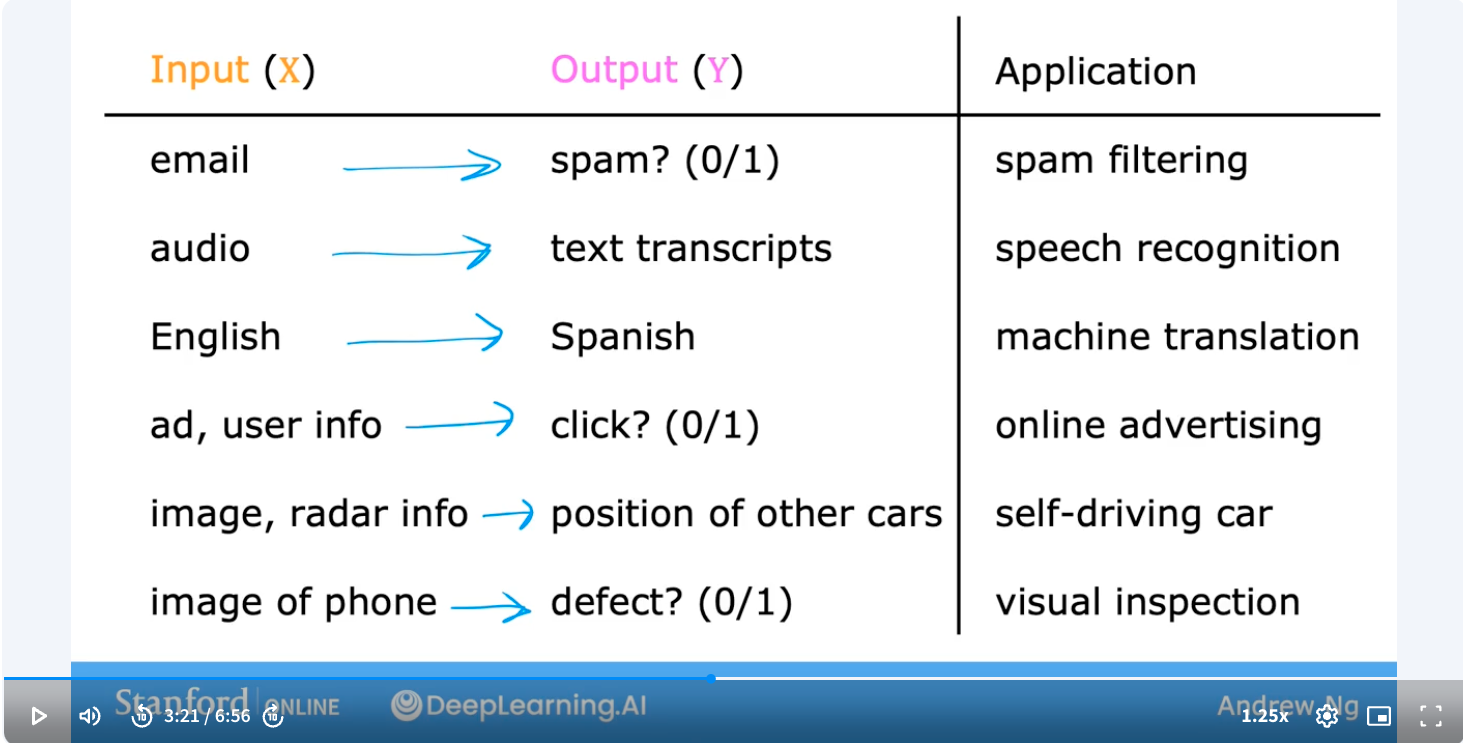
\includegraphics[height=5.3cm]{course_img/supervised_ex}
\end{definitionbox}

\begin{examplebox}
	\textbf{Regression}--- Predicting a number with a continous set of outputs.
	\begin{itemize}
		\item Fit some input data to evaulate the house price using the best fit 
		\item Learn about ML algorithms to pick the best evaluating tool, e.g., linear or quadratic model 
	\end{itemize}		
	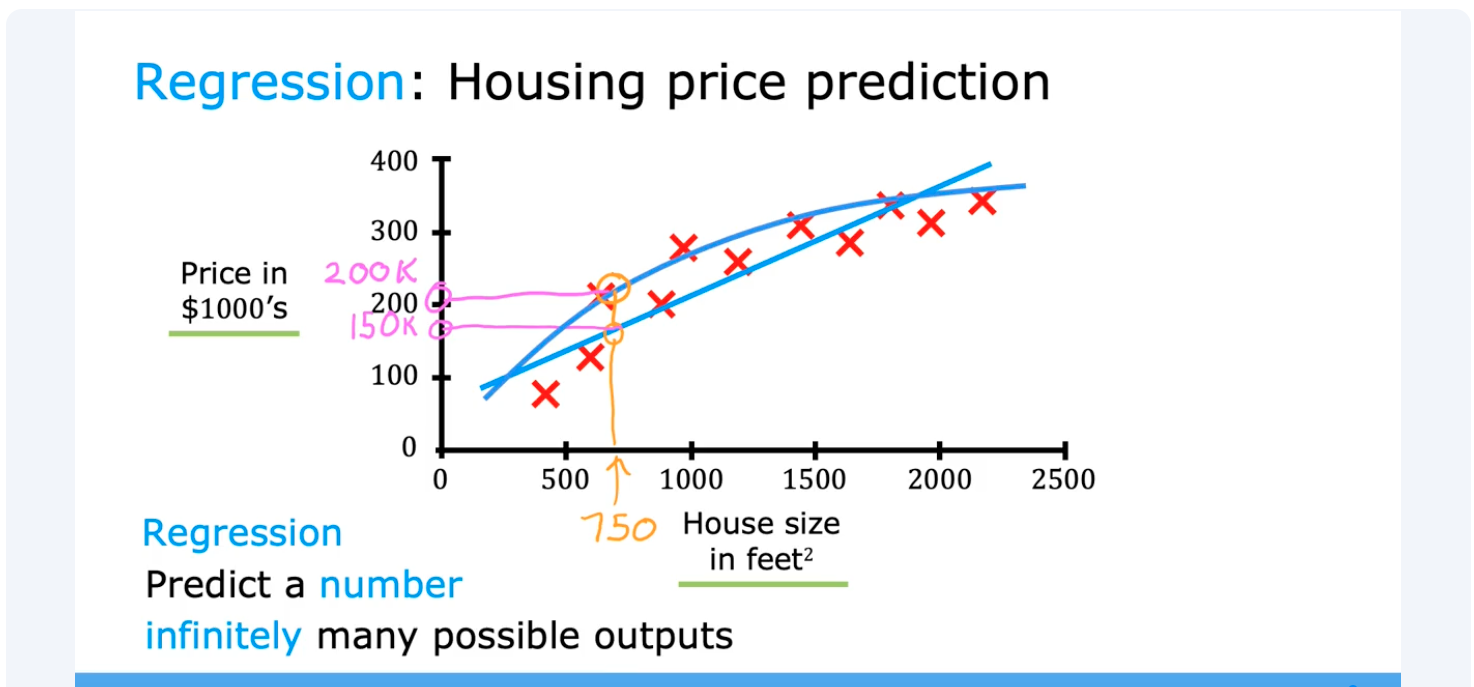
\includegraphics[scale=0.2]{course_img/regression_ex}
\end{examplebox}

\begin{examplebox}
	\textbf{Classification}--- Predicting a value from a finite set of possible outputs, e.g., benign(0) or malignent(1) tumor based on some input data (tumor size)
	\begin{itemize}
		\item Class or category used interchangeably for output value
		\item Can have multiple inputs (right image) where the ML algorithm forms a boundary on multi-dimensiinal data to predict the classification 
	\end{itemize}
	\begin{minipage}[c]{\textwidth}	
		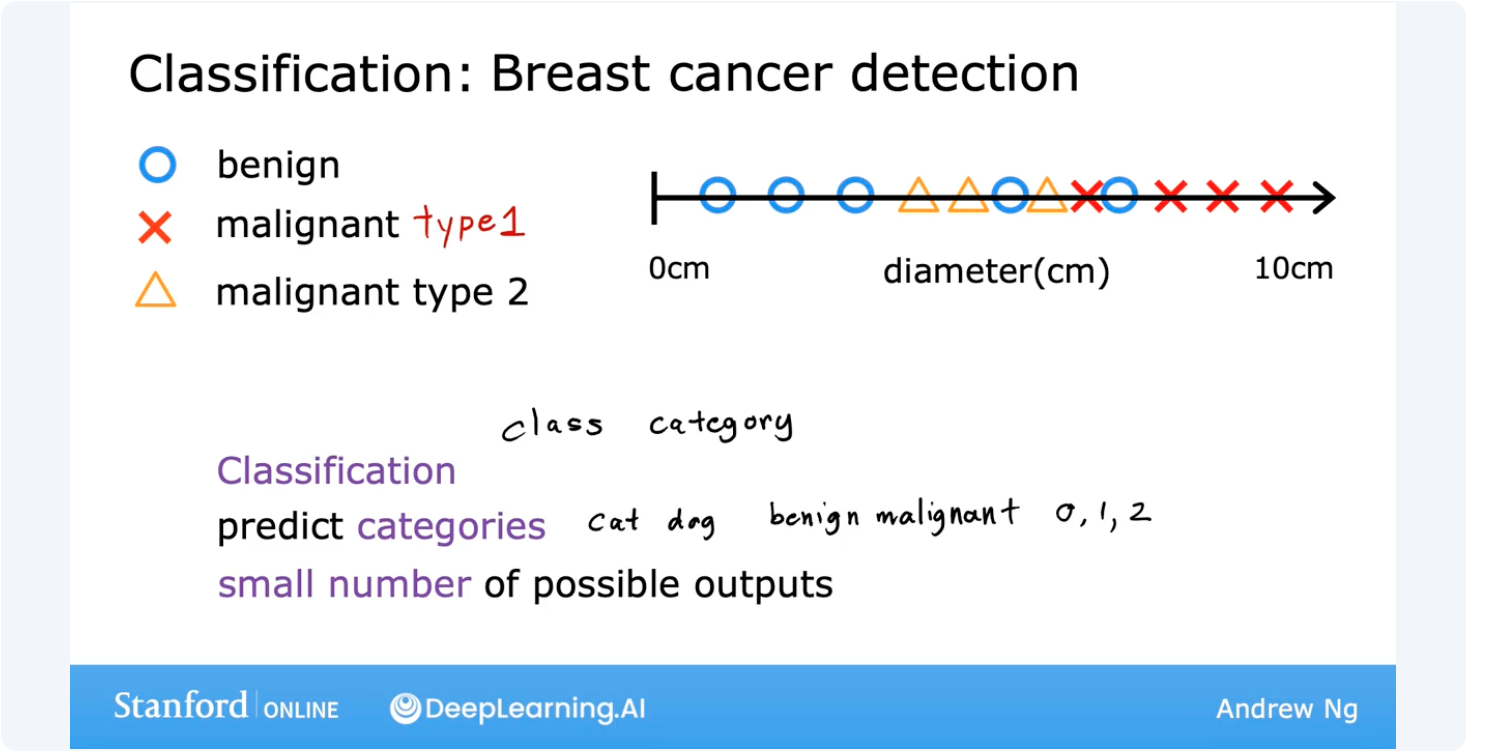
\includegraphics[width=.69\textwidth]{course_img/classification_ex}
		\hfill
		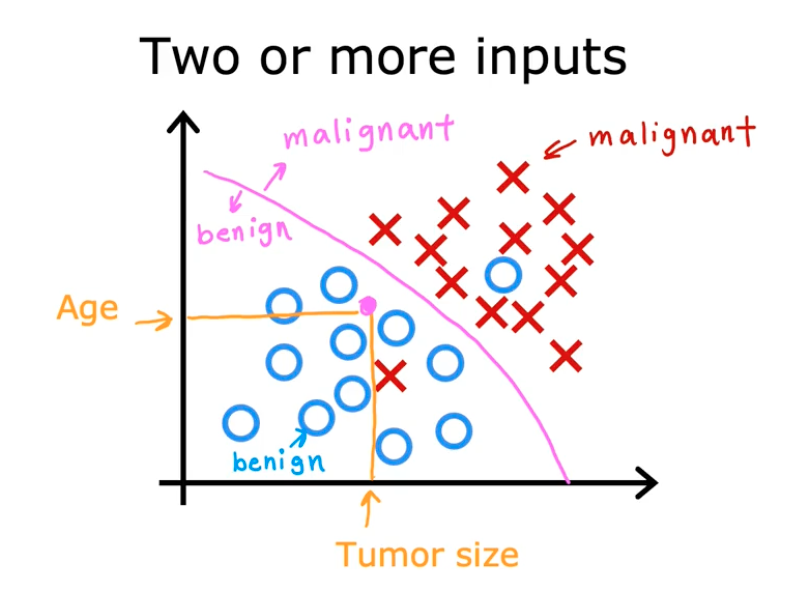
\includegraphics[width=.29\textwidth]{course_img/classification_ex2}
\end{minipage}			
\end{examplebox}

\subsection{Unsupervised Learning}

\begin{definitionbox}
	\textbf{Unsupervised Learning}---  Find patterns or structures in unlabeled data
	\begin{itemize}
		\item \textit{Clustering}: group unlabeled data 
		\item \textit{Anomaly detection}: detect ambigious or outliers in data
		\item \textit{Dimensionality reduction}: compress large data sets into smaller ones without loosing the important information 
	\end{itemize}
\end{definitionbox}

\begin{examplebox}
	\textbf{Clustering}--- groups data into clusters that have similar characteristics
	\begin{itemize}
		\item google news example clusters articles by similar keywords in article titles to group similar stories
		\item dna grouping for types of people
		\item grouping customers with similar goals to predict best suggestions
	\end{itemize}
	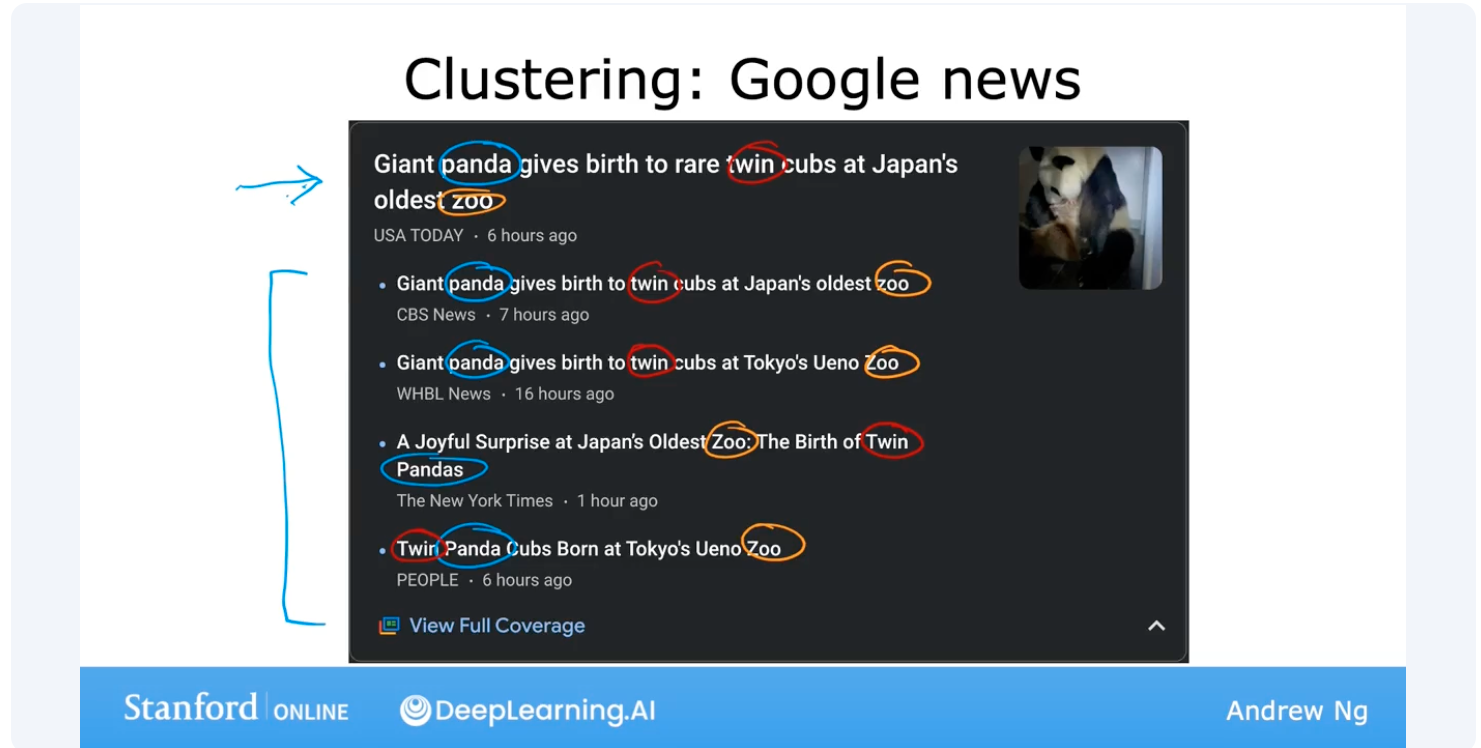
\includegraphics[width=0.6\textwidth]{course_img/clustering_ex}
\end{examplebox}

\subsection{Linear Regression}

\begin{definitionbox}
	\textbf{Training Set}: data used to train the model consisting of $m$ input ($x^i$) and output ($y^i$) variables with ($x^i,\ y^i$) as the ith training point.
	\\
	\textbf{Learning Algorithm}: Takes the training set and outputs a function to predict the output ($\hat{y}$) from the input feature, ($x$), e.g., 
	\[
		x \rightarrow \boxed{\textcolor{blue}{f}} \rightarrow \textcolor{red}{\hat{y}} 
	\]
\end{definitionbox}

\begin{notebox}
	For supervised learning the training set contains the `correct output' ($y$), not to be confused with the estimated output from the model ($\hat{y}$)
\end{notebox}

\begin{itemize}
	\item Most widely used ML model in real world applications, e.g., 
	\item For linear regression the function or model, $\textcolor{blue}{f}$, is a linear funtion:
	\begin{equation}\label{eq:linearRegression}
		f(x) = wx+b
	\end{equation}	 
	 where $w,\ b$ are parameters of function.
	\item Foundational model for estimating outputs, also called \textbf{univariante} linear regression (one variable) and basis for more complex models, e.g., quadratic.
\end{itemize}

\subsection{Cost Function}

\begin{definitionbox}
	\textbf{Cost Function} tells us how good the model fits to the data and can be expressed in many forms, see example of squared error cost function $J(w,b)$., and can be minimized to find the best parameters for the model.
	\begin{equation}\label{eq:cost_function}
		J(w,b) = \frac{1}{2m} \sum_{i=1}^m \left( f_{w,b} \left( x^{(i)} \right) - y^{(i)} \right)^2
	\end{equation}
\end{definitionbox}

\begin{examplebox}
	\begin{itemize}
		\item Squared error cost function compares the predicted value ($\hat{y}$) from the linear model $f(x)=w\cdot x + b$ to the true value ($y$).
	\end{itemize}
	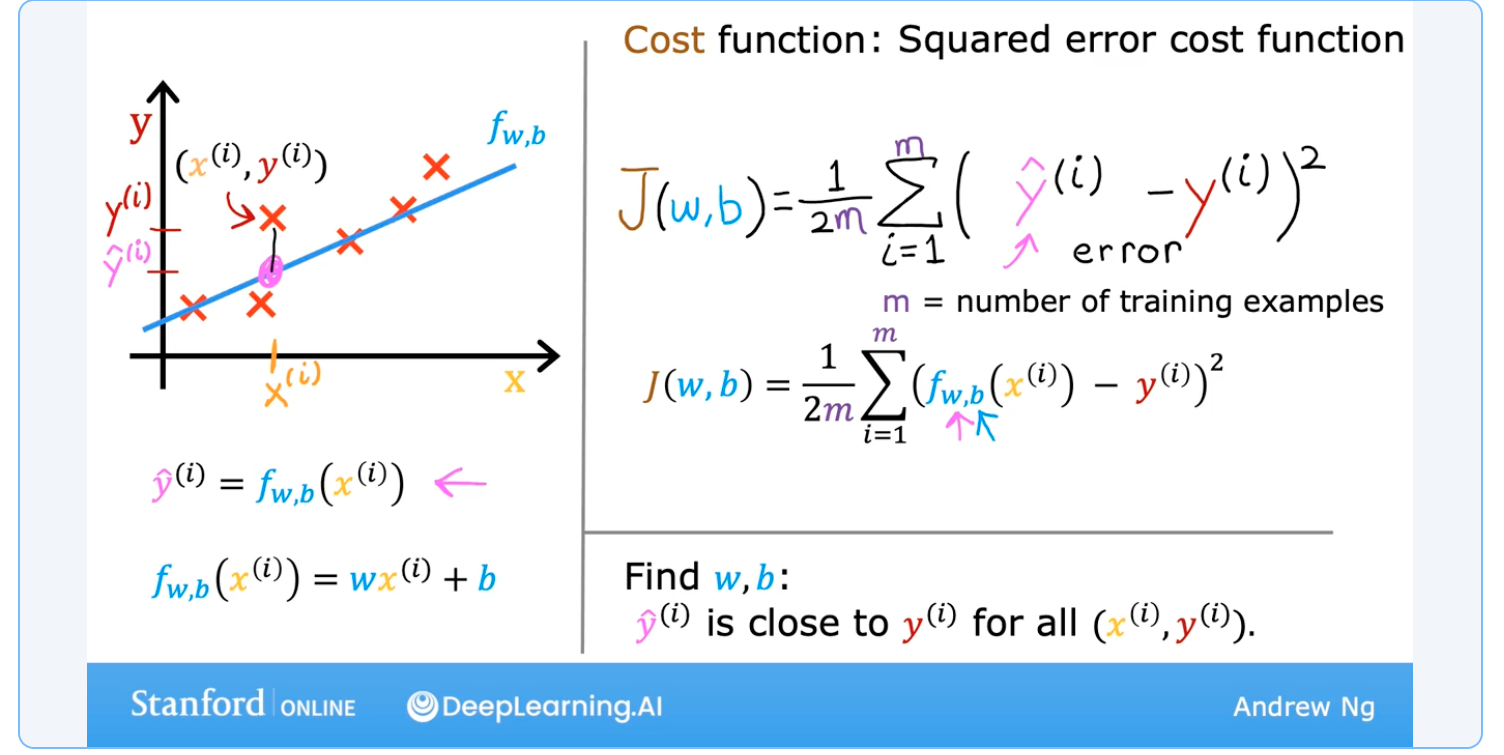
\includegraphics[height=5cm]{course_img/costfunction_ex}
\end{examplebox}

\subsubsection{Parameter Estimation with Cost Function}

\begin{examplebox}
	\begin{itemize}
		\item By minimizing the Cost Function we can get best parameters that fit our data 
		\item The example below used simplified linear model with no bias ($b=0$) and the squared error cost function  
		\item We see the parameter that minimized J (smallest value) $J(1)$ gives the best fit to the data.	
		\begin{equation}
			J(w) = \frac{1}{2m} \sum_{i=1}^m \left( f_w \left( x^{(i)} \right) - y^{(i)} \right)^2
			= \frac{1}{2m} \sum_{i=1}^m \left( wx^{(i)} - y^{(i)} \right)^2 
		\end{equation}
	\end{itemize}
	\begin{minipage}{\textwidth}
		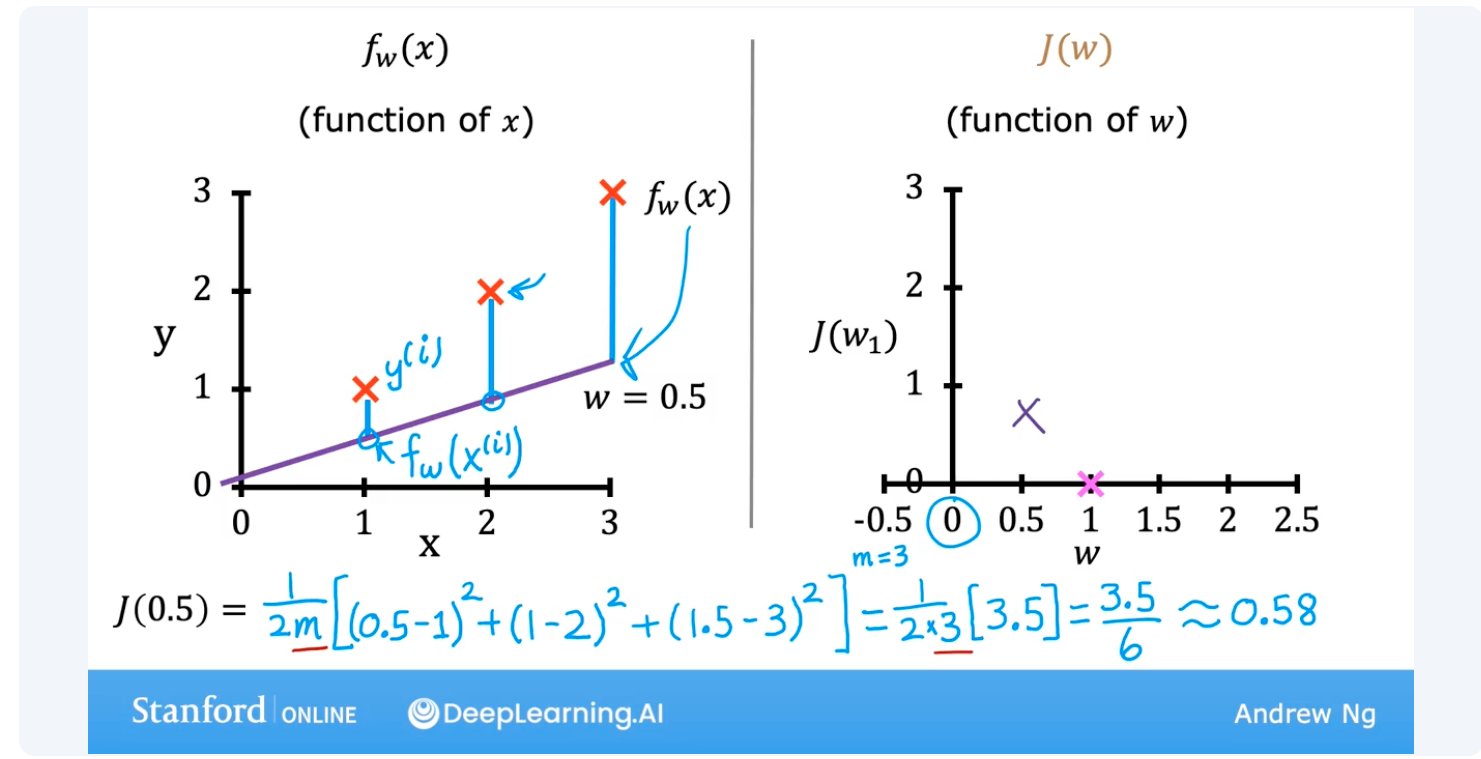
\includegraphics[width=.49\textwidth]{course_img/evaluate_cost_ex}
		\hfill
		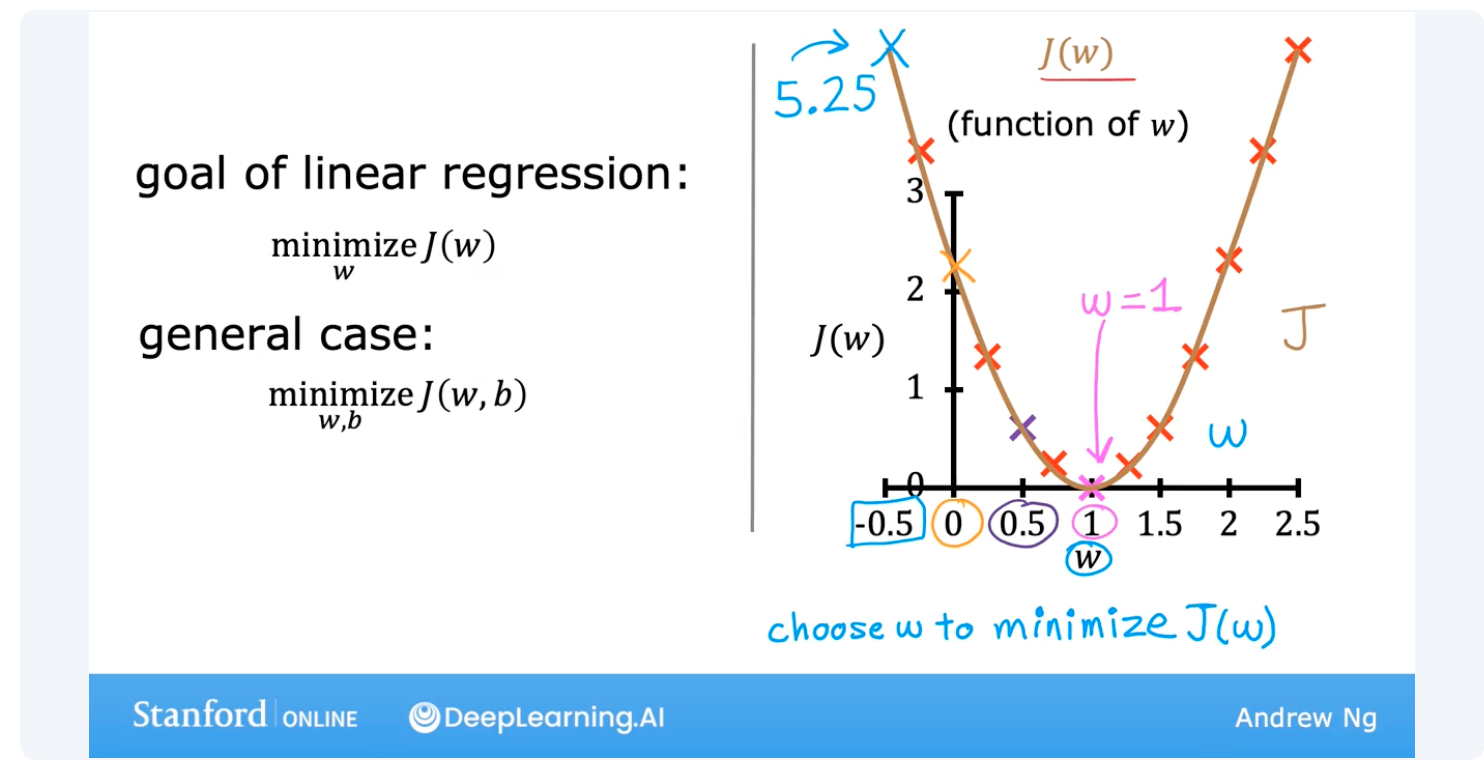
\includegraphics[width=0.49\textwidth]{course_img/minimize_cost_simple_ex}	
	\end{minipage}
	\\
	\begin{itemize}
		\item For the complex function with multiple parameters (2 in this example) the cost function is is a 3D plot and can be visualized as a contour plot to estimate many parameters.
		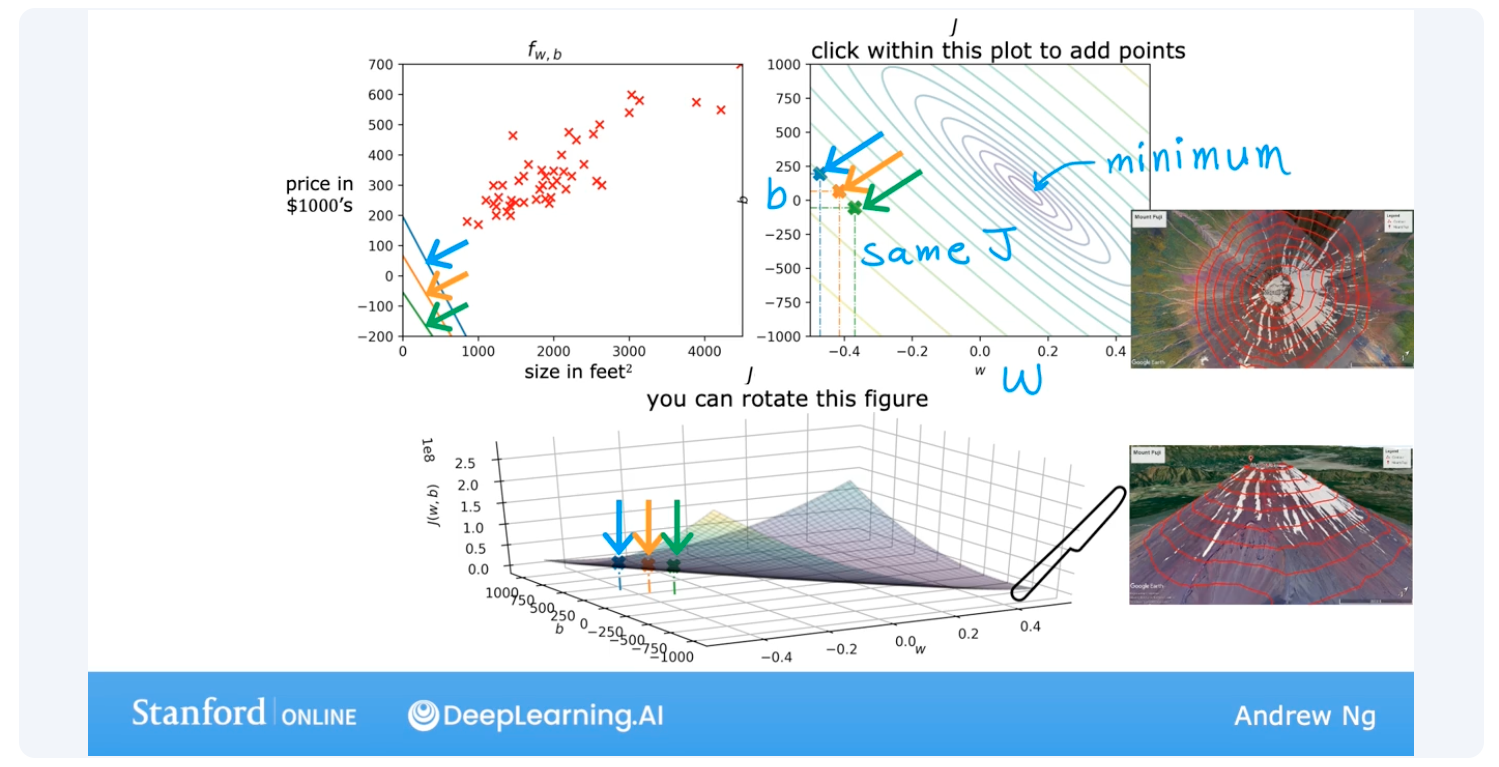
\includegraphics[height=5cm]{course_img/2dcost_contour_ex} 
	\end{itemize}
\end{examplebox}
	
\subsection{Gradient Decent}

\begin{definitionbox}
	\textbf{Gradient Decent} is an algorithm used to minimize any functions including the cost function discussed by taking steps towards the greatest decent of the function.
	\begin{align}
		w &\coloneq w -\alpha \frac{\partial}{\partial w}J(w,b) 
		 \nonumber \\
		b &\coloneq b -\alpha \frac{\partial}{\partial b}J(w,b) \label{eq:gradinet_descent_linear}
	\end{align}
	where $\alpha$ is the `learning rate' that dictates the size of the steps and the equations above are updated simultaneously for two-parameter cost function by reassigning the parameter value at each step.
\end{definitionbox}

\begin{notebox}
	The \textbf{Gradient Term} in the above set of equations determines whether the parameter is decreasing or increased based on the slope of the cost function $\frac{\partial}{\partial w}J(w,b,..)$ for all parameters until the parameters reach a local/global minimum. 
	\begin{align}
		\frac{\partial}{\partial w}J(w,b,..) &> 0\quad  \therefore \quad w_{new} < w \\
		\frac{\partial}{\partial w}J(w,b,..) &> 0\quad \therefore  \quad w_{new} >w 		
	\end{align}
\end{notebox}

\begin{notebox}

	\textbf{Learning rate} must be chosen to optimize speed of algorithm and likelihood of convergence:

	\begin{wrapfigure}{l}{0.3\textwidth}
		\centering		
		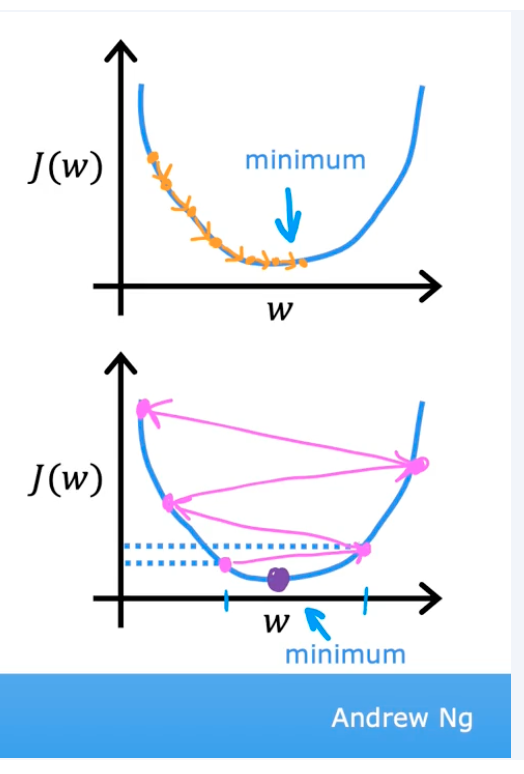
\includegraphics[width=0.24\textwidth]{course_img/learning_rate_ex}
	\end{wrapfigure}

	How learning rate affects minimization:
	\begin{itemize}
		\item If the learning rate is too small the algorithm is extremely slow and inefficient. (Top image with tiny steps)
		\item If the learning rate is too large then the algorithm could fail by missing the minimum or fail to converge. (Bottom image with massive steps)
		\item Near a local minimum the slope(rate of decesnt) becomes smaller and thus the parameters change by smaller values so with a fixed $\alpha$ the `steps' become smaller
	\end{itemize}
	\vspace{1cm}
	
\end{notebox}

\subsubsection{Implementation}

\begin{itemize}
	\item Correct implementation of simultaneously updating parameters (skeleton code)
	\item The updating of the parameters must be done after the determination of the new parameters using the previous ones first.	
\end{itemize}
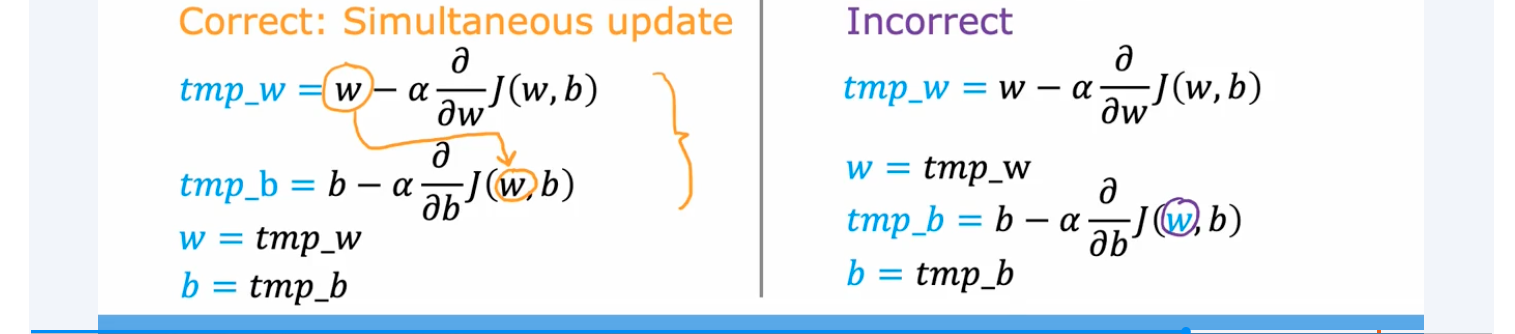
\includegraphics[width=0.9\textwidth]{course_img/implement_gradientDesent_ex}

\begin{examplebox}
	Lets apply gradient decent~(\cref{eq:gradinet_descent_linear}) to the linear regression	 model~(\cref{eq:linearRegression}) parameters using the squared errors cost function~(\cref{eq:costFunction}). The gradient decent algorithm then decomposes to multiple iterations of the solutions of the parameters with some initial guess ($w,b$):	
	\begin{align}
		w' &= w - \alpha \left[ \frac{1}{m} \sum _{i=1}^{m} \left( f_{w,b}(x^{(i)})-y^{(i)} \right)x^{(i)}  \right] 		
		\\
		b' &= b - \alpha \left[ \frac{1}{m} \sum _{i=1}^{m} \left( f_{w,b}(x^{(i)})-y^{(i)} \right)  \right]
	\end{align}
	where the bracket terms have been evaluated and are the partial derivatives of the cost function with the linear regression model.
\end{examplebox}

\begin{notebox}
	\begin{itemize}
		\item When solving for more complex cost functions, the gradient decent algorithm can lead to different paths and get `stuck' in local minima, depicted below:\\ \\
	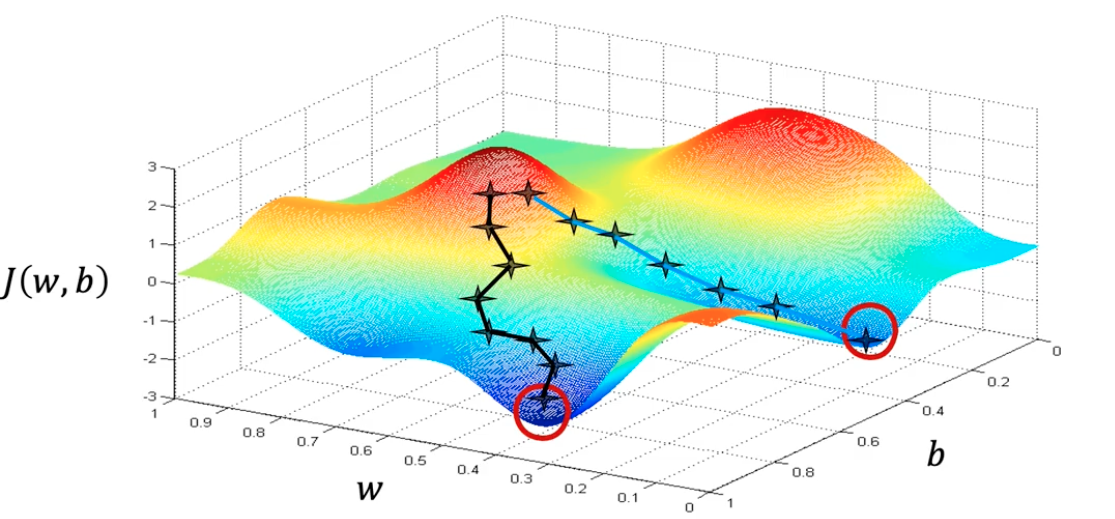
\includegraphics[height=5cm]{course_img/gradient_decent_manymin}
	\item The special case of the squared errors cost function take a bowl shape and only has a single global minimum.
	\end{itemize}		
	
\end{notebox}


\newpage
\section{Week 2: Regression with multiple input variables}

\subsection{Overview}
- Key objectives  
\begin{itemize}
	\item Vectorization
	\item Gradient decent for multiple linear regression (many features,  $x_i$) 
	\item Feature Scaling
	\item Feature Engineering
	\item Polynomial Regression
	
\end{itemize}

\noindent 
- Implementation
\begin{itemize}
	\item Checking gradient decent convergence
	\item choosing learning rate
	\item Using scikit-learn for gradient descent and regression models
\end{itemize}

\begin{notebox}
	\textbf{Multiple Features} or inputs to your training sets are defined as $x_j^{(i)}$, where their can be $n$ features/input values for i\textsuperscript{th} training sample. 
	\\ 
	\textbf{Multiple Linear Regression} is then a linear regression model with multiple features and can be written in terms of vectors
	\begin{equation}\label{eq:multiple_linear_regression}
		f_{\vec{w},b} = \vec{w}\cdot \vec{x} + b,
	\end{equation}
	where the vector is a list of values defined in the normal way $\vec{v}=(v_1,\ v_2,\  \dots v_n)$ and the dot product is defined as the sum of the product of each vector element-wise
	\begin{equation}\label{eq:dot_product}
		\vec{a}\cdot \vec{b} = \sum\limits_{i=0}^{n-1} a_i b_i
	\end{equation}
\end{notebox}

\subsection{Vectorization}

\begin{itemize}
	\item Make code shorter and more efficient
	\item Take advantage of modern linear algebra libraries and gpu hardware using parallel processing to scale to large data sets
	\item Use arrays in NumPy python library, e.g.,  \verb|w = np.array([1.0,2.5,-3.3])|
\end{itemize}

\begin{notebox}
	\textbf{Broadcasting} is how numpy treats arrays of different sizes by means of vectorizing array operations in C instead of python (\href{https://numpy.org/doc/stable/user/basics.broadcasting.html}{documentation})
\end{notebox}
\begin{examplebox}
	-- Implementation of vectors for processing where the dot product is standardized with built-in NumPy methods.\\
	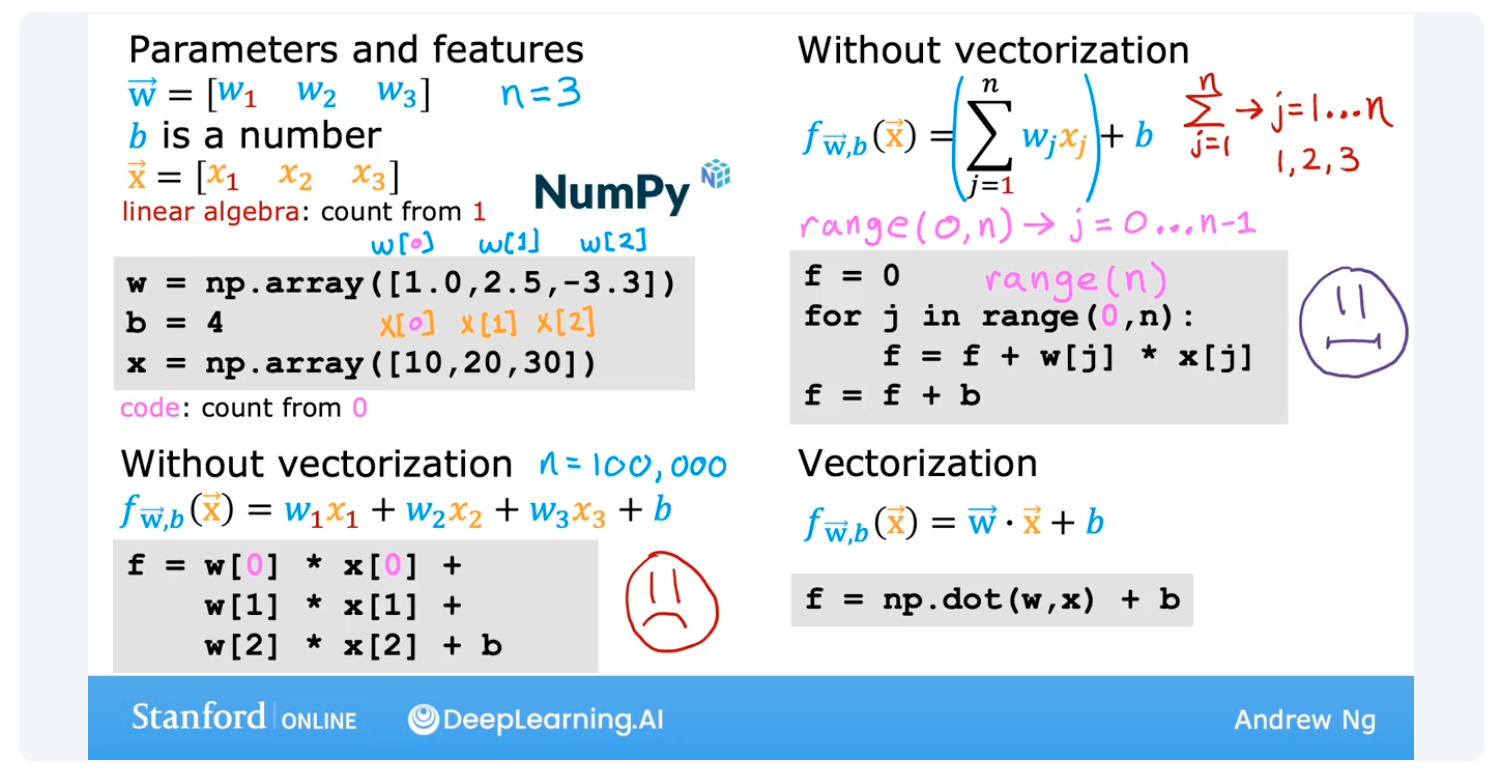
\includegraphics[height=5cm]{course_img/numpy_vector_ex}
	
	-- Implementation of vectorization in gradient decent for 16 parameter linear regression \\
	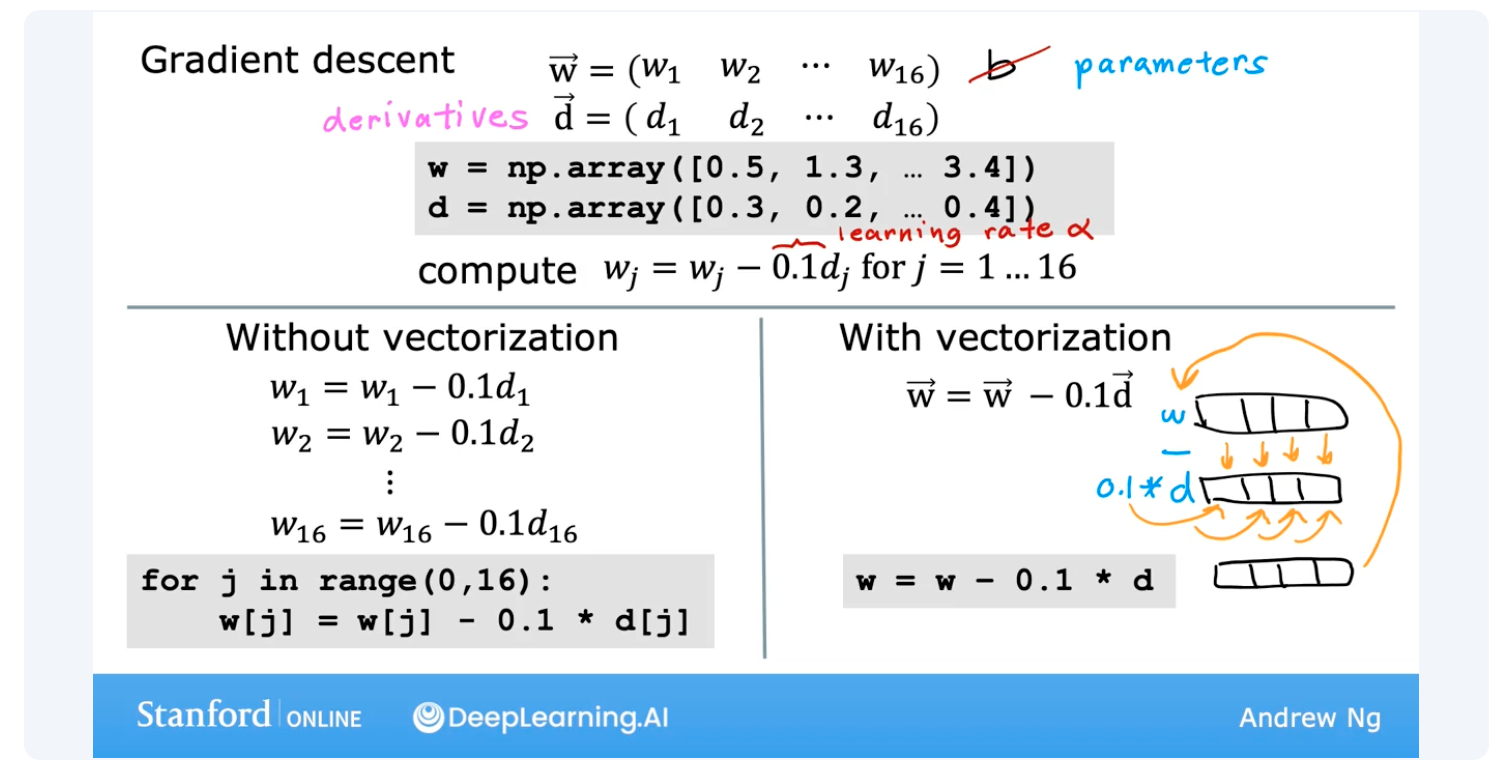
\includegraphics[height=5cm]{course_img/gradient_decent_vector_ex}
\end{examplebox}

\subsubsection{Gradient Decent with vectorization}

\begin{definitionbox}
	-- vector notation
	\begin{align}
		\textbf{ Parameters}& \quad \vec{w}=[w_1 \dots w_n \nonumber \\
		\textbf{ Model}& \quad f_{\vec{w},b}=\vec{w}
		\cdot \vec{x} +b \nonumber \\
		\textbf{Cost Function}& \quad J(\vec{w},b) \nonumber \\
		\textbf{ Gradient Decent}& \quad \text{repeat} 
		\begin{cases}
			w_j = w_j -\alpha \frac{\partial}{\partial w_j}J(\vec{w},b) &	\\
			b = b  -\alpha \frac{\partial}{\partial b}J(\vec{w},b)
		\end{cases} \label{eq:gradient_descent_multi}
	\end{align}
	
	-- Gradinet decent with square errors cost function for multiple linear regression then becomes
	\begin{equation}\label{eq:gradient_decent_multi_linear}
		\text{repeat}
		\begin{cases}
			\vec{w} = \vec{w} - \alpha \frac{1}{m}\sum\limits^{m}_{i=1} \left( f_{\vec{w},b}(\vec{x}^{(i)})-y^{(i)}\right) \vec{x}^{(i)} &	\\
			b = b  -\alpha \frac{\partial}{\partial b}\frac{1}{m}\sum\limits^{m}_{i=1} \left( f_{\vec{w},b}(\vec{x}^{(i)})-y^{(i)}\right)
		\end{cases} ,
	\end{equation}
	where each component of feature $w_j$ is compactly written as a vector $\vec{w}$ and each feature is simultanously updated along with b.
\end{definitionbox}

\begin{notebox}
	\textbf{Normal Equation} can be used for linear regression as an alternative to gradient decent where linear algebra libraries can solve for the best parameters in one go instead of through many iterations.\\
	--Disadvantages:
	\begin{itemize}
		\item Only useful for linear regression and does not generalize to other learning algorithms
		\item Slow for large number of features ($>$10k)
	\end{itemize}
\end{notebox}

\subsection{Feature Scaling}

\begin{definitionbox}
		\textbf{Feature Scaling} is an algorithm that allows for the scaling of features of your model  to speed up gradient decent.
		\begin{itemize}
			\item scaling of parameters typically proportional to range of feature, e..g., a feature that spans $(0,5)$ will have a larger scaling than a feature ranging $1000-5000$ (intuitive)
			\item The feature scaling allows for the values of your equations to have similar scaled values and is important for the gradient decent algorithm spacing to run smoothly, e.g., the phase space of parameters with vastly different ranges is difficult to analyze efficiently (shown by the contour plots below)
		\end{itemize}
		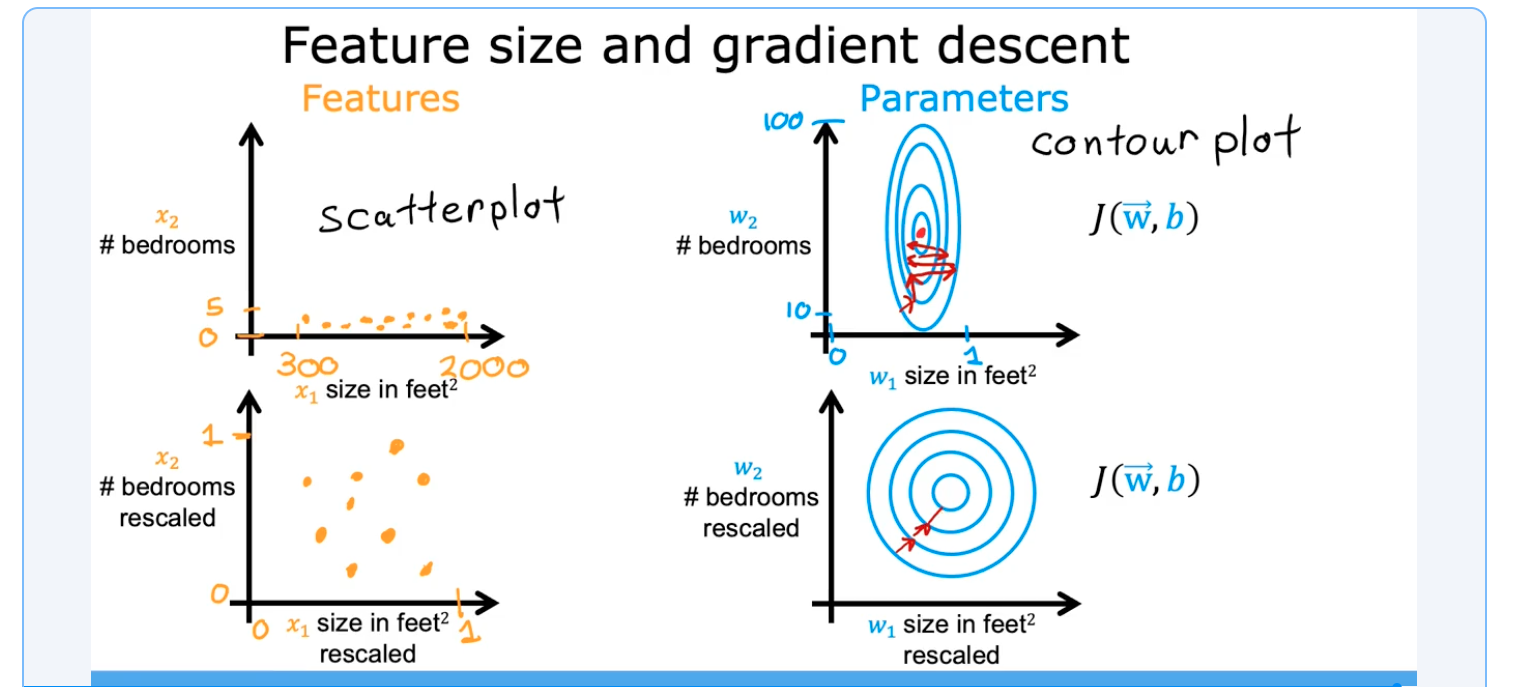
\includegraphics[height=6cm]{course_img/feature_scaling_ex}
\end{definitionbox}

\begin{examplebox}
	-- \textbf{Maximum normalization}  scales features in your model by the maximum value of the range to force them to be in smaller range, e.g., $(min,1)$:
	\begin{equation}
		x_{i,\,scaled} = \frac{x_i}{max\{x_i\}}
	\end{equation}
	where $max{x}$ is just the maximum value of the feature.
	\\
	-- \textbf{Mean normalization} scales the features by the mean of the feature ($\mu_i$):
	\begin{equation}
		x_{i,\,scaled} = \frac{x_i - \mu_i}{R_{x_i}}
	\end{equation}
	where the range of the feature is labeled $R_{x_i} \equiv max\{x_i\}- min\{x_i\} $. \\
	This choice of scaling will range from $(-1,1)$ and is a symmetric range.
	\\
	-- \textbf{Z-score normalization} scales the feature by using the standard deviation $\sigma_i$ of the feature:
	\begin{equation}
		x_{i,\,scaled} = \frac{x_i - \mu_i}{\sigma_i}
	\end{equation}
	where the standard deviation gives us a measure of the spread of the data in statistics. 
\end{examplebox}

\subsection{Convergence of gradient decent}

\begin{definitionbox}
	\textbf{Learning Curves} give an indicator of how the algorithm is working over the evolution of iterations in the case of minimizing the cost function (example below).  \\
	\indent -- Can take many forms for different applications in ML 
\end{definitionbox}

\begin{examplebox}
	-- Plot a learning curve where the cost function is plotted against the \# of iterations (below) \\
	-- The learning curve should be a smooth descending function, converging to singular value.
	\begin{itemize}
		\item If not than its a sign that the learning rate $\alpha$ may be too large (example where we pass the minima)
	\end{itemize}
	-- Also give a feel for the number of iterations needed to converge \\
	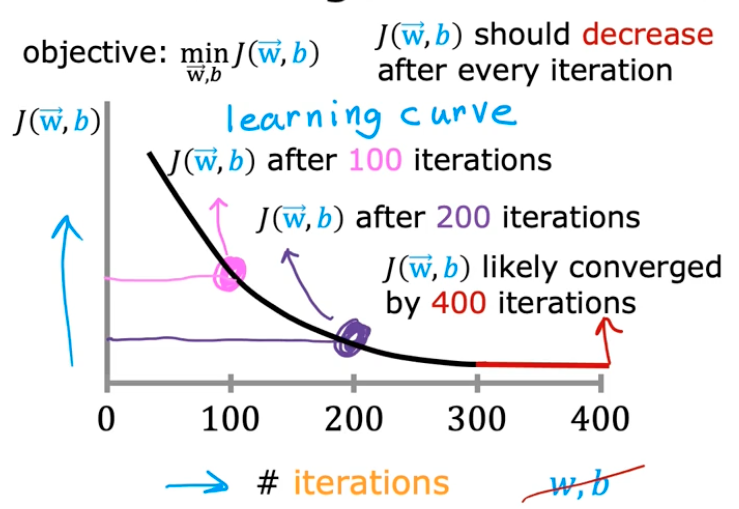
\includegraphics[height=6cm]{course_img/learning_curve_ex}
\end{examplebox}

\begin{notebox}
	-- Can also rely on automatic convergence tests where:
	\begin{quote}
		Let $\epsilon$ be a small number, e.g.,$10^-3$ \\
		If $J(\vec{w},b)$ decreases by $\leq \epsilon$ in one iteration than we declare convergence
	\end{quote}
	
	-- Its usually still useful to illustrate the convergence with learning curves
\end{notebox}

\subsubsection{Choosing Learning Rate}

\begin{notebox}
	\begin{itemize}[leftmargin=*]
		\item By looking at the leaning curve we can verify that the cost
	 function is smoothly decreasing and the learning rate is not too large.
		\item By looking at the rate of the decent for convergence of the cost function we can adjust the learning rate to be more efficient without being too small.
		\item If the learning curve is always increasing than we may have a bug in our code
	\end{itemize}	
\end{notebox}

\subsection{Feature Engineering}

\begin{definitionbox}
	\textbf{Feature engineering} is the practice of designing new features by  transforming or combining original features that could be better predictors for the model, e.g., for house prices given the frontage ($x_1$) and depth ($x_2$) of the lot the area ($x_3=x_1x_2$) can be defined and used in the model, where
	\[ 
	f_{\vec{w},b}(\vec{x}) = w_1x_1+w_2x_2+w_3x_3 +b
	\]
to improve the model.
\end{definitionbox}

\subsection{Polynomial regression}

\begin{definitionbox}
	\textbf{Polynomial regression} is a model to fit non-linear data such as polynomial functions of different orders, e.g., a polynomial regression to $n$ order,
	\begin{equation}
		f_{\vec{w},b}(\vec{x}) = w_1x+w_2x^2+w_3x^3 + \dots + w_nx^n +b
	\end{equation}
	where a cut off can be made to best fit the data.\\
	
	-- Have to be particularly careful to use feature scaling because now the size of each term grows quadratic in the feature. 
	
\end{definitionbox}
	
\begin{examplebox}
	
	Choice of features to use when feature engineering using polynomial regression:\\
	-- polynomial to the second ($x^2$) or third power ($x^3$) for a feature,e.g., price vs house sizes below \\
	
	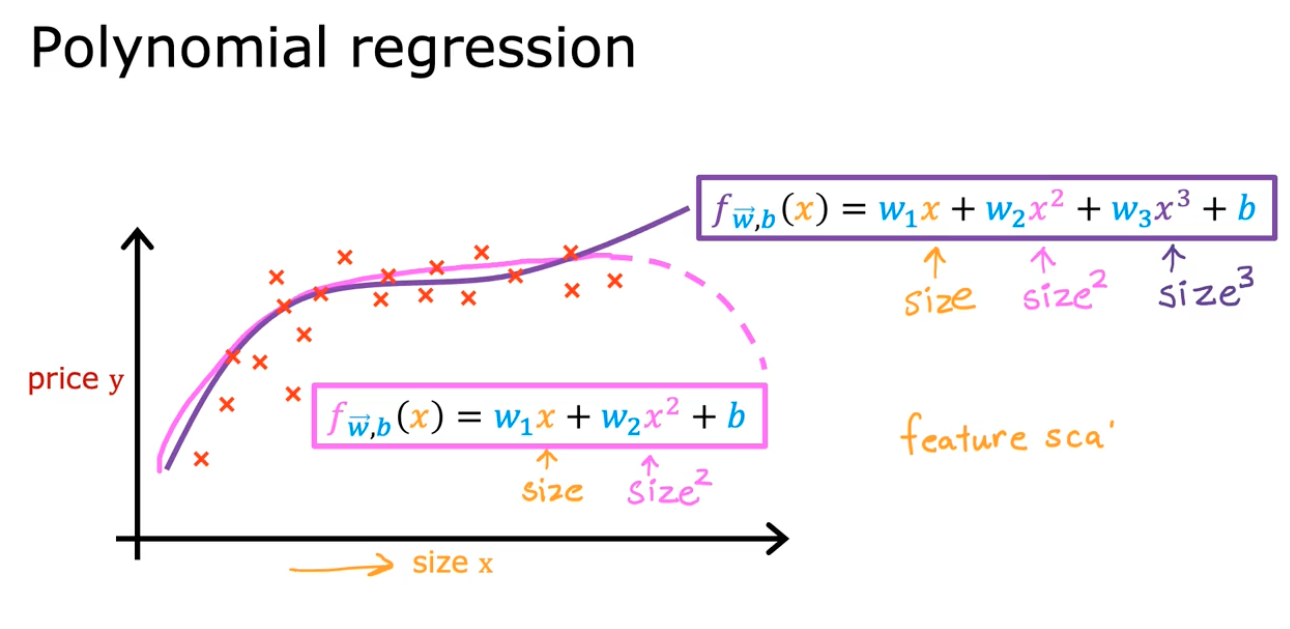
\includegraphics[height=6cm]{course_img/polynomial_regression_ex}	
	
	-- polynomial with power $1/2$ ($\sqrt{x}$) for a monotonically increasing fit \\
	
	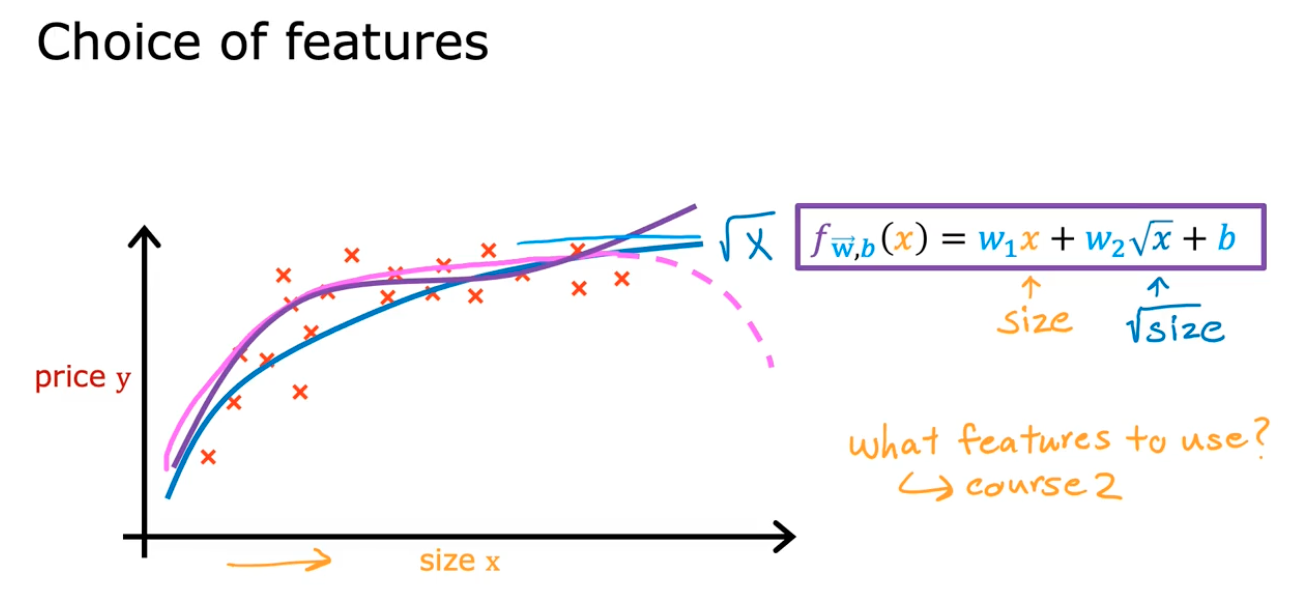
\includegraphics[height=6cm]{course_img/polynomial_reg_sqrt}
\end{examplebox}

\newpage
\section{Week 3: Classification}

\subsection{Overview}
- Key objectives  
\begin{itemize}
	\item Classification 
	\item Logistic regression
	\item Decision Boundary
	\item Overfitting
	\item Regularization
\end{itemize}

\noindent 
- Implementation
\begin{itemize}
	\item Sigmoid function 
	\item Cost function for logistic regression
	\item Gradinet descent for logistic regression
	\item Regularized linear regression
	\item scikit-learn implementation
\end{itemize}

\begin{definitionbox}
	\textbf{Binary classification}  have two potential outputs, e.g., (yes,no), (tue(1),false(0))
	\begin{itemize}
			\item `Negative' class (false) vs `Positive' class (true) where class/category is interchangeable for outputs
	\end{itemize}
\end{definitionbox}

\begin{notebox}
	Linear regression is no longer a good model for classification where we see how fitting a binary data set leads to misrepresentation of the predictions below,e.g.,\\
	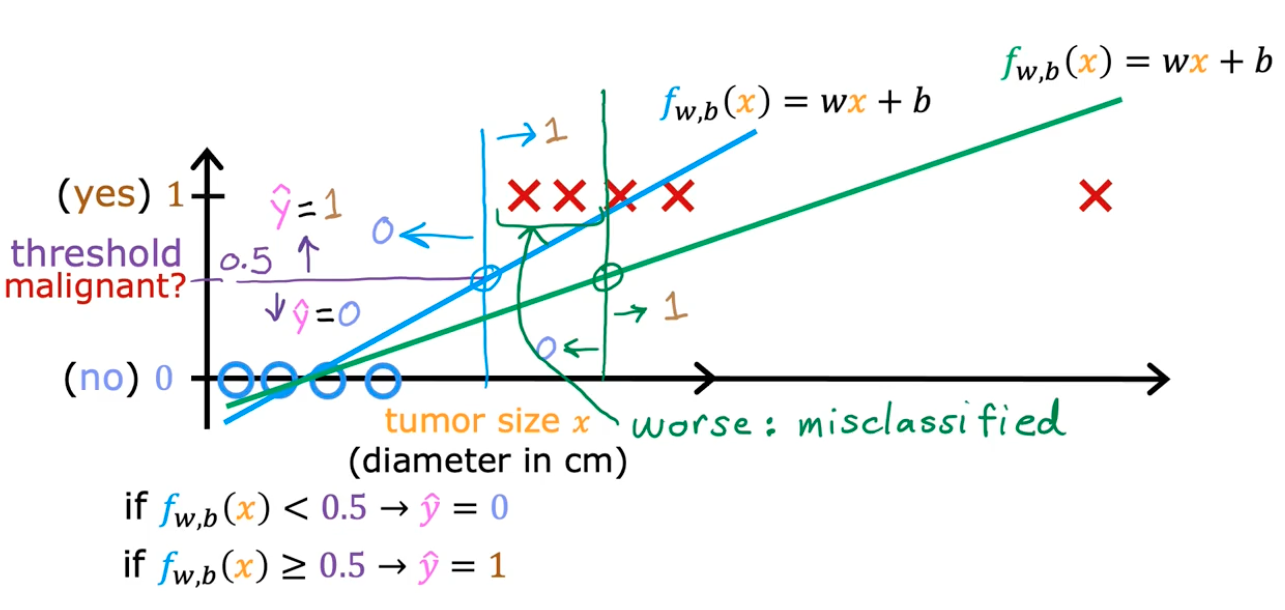
\includegraphics[height=5cm]{course_img/linear_reg_classification_ex}
\end{notebox}

\subsection{Logistic Regression}
	
\begin{definitionbox}
	\textbf{Sigmoid/logisitic function} is a function that gives an output of 0 or 1 and is valuable for modeling two-level systems represented by:
	\begin{equation}\label{eq:sigmoid}
		g(z) = \frac{1}{1+e^{-z}} \quad 0 < g(z) < 1.
	\end{equation}
	A visual representation of the function is:\\
	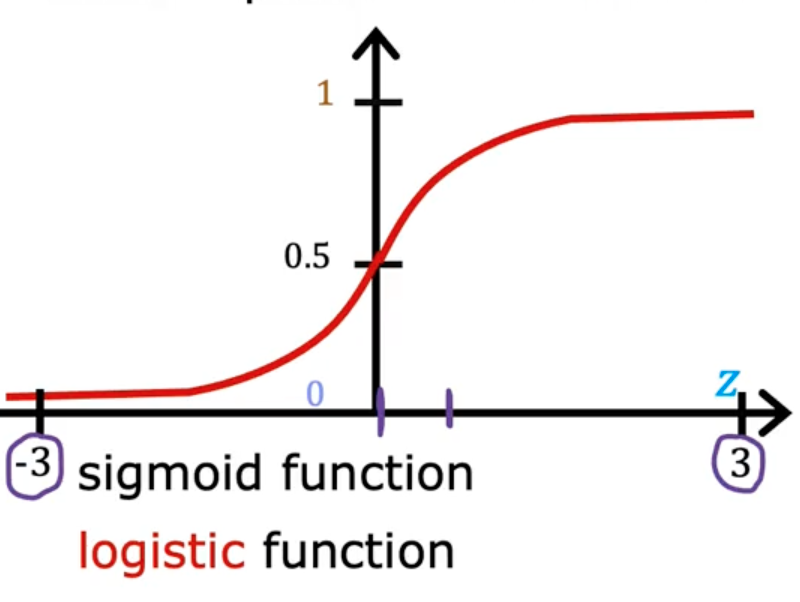
\includegraphics[height=5cm]{course_img/sigmoid_ex}
	
\end{definitionbox}

\begin{notebox}
	\textbf{Logisitic Regression} model is written in terms of the sigmoid function~(\cref{eq:sigmoid}) where our independent variable $z$ is represented by a linear function of our feature $\vec{x}$:
	\begin{equation}
		z = \vec{w}\cdot \vec{x} + b.
	\end{equation}
	This transformation is used to construct the logisitc regression model:
	\begin{equation}\label{eq:logistic_regression}
			f_{\vec{w},b}(\vec{x})=g(\vec{w}\cdot \vec{x} + b) = \frac{1}{1+\exp \left[ -(\vec{w}\cdot \vec{x} + b)\right] }
	\end{equation}
	\begin{itemize}
		\item The linear rergression algorithm outputs a value from (0,1) and thus acts like a probability to determine the classification and can be written technically as:
		\begin{equation}
			f_{\vec{w},b}(\vec{x}) = P(y=1|\vec{x};\vec{w},b)
		\end{equation}
		that says what is the probability of $y=1$ for the feature $\vec{x}$ given the values of $\vec{w},b$.
	\end{itemize}
\end{notebox}

\subsubsection{Decision Boundary}

\begin{definitionbox}
	The \textbf{Decision Boundary} is the threshold of the model to predict a binary result either true or false and can be defined when the transformed variable $z=0$, e.g., for the linear regression this would be $z=\vec{w}\cdot \vec{x} + b =0$ and represents when the decision is not quit 0 or 1.
	\begin{itemize}
		\item Due to the continuous nature of the sigmoid function where recall the outputs can take any value (0,1) interpreted as a probability. \\
		\item The typical threshold is for the model is $\leq 0.5$ whether the results are predicted true or false
	\end{itemize}
\end{definitionbox}

\begin{examplebox}
	We look at a simple example with two features and transform our \textbf{multiple linear regression} to logistic regression using~\cref{eq:logistic_regression}, so now the function takes the form:
	\begin{equation}
		f_{\vec{w},b}(\vec{x}) = g(w_1x_1+w_2x_2 +b).
	\end{equation}
	To find the decision boundary we solve for $z=0$ with parameters $\vec{w}=(1,1),\ b=-3)$ for the above model to get the boundary~\cref{eq:boundary_ex}:
	\begin{gather}
		z=x_1 + x_2 - 3 = 0 \nonumber \\
		x_1 + x_2 = 3 \label{eq:boundary_ex}
	\end{gather}
	and represented in the below figure, where the boundary is depicted\\
	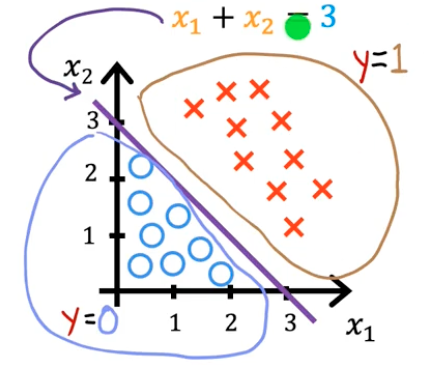
\includegraphics[height=5cm]{course_img/decision_boundary_ex}
\end{examplebox}

\begin{examplebox}
 	We can also look at a \textbf{non-linear decision boundary} with two features with the underlying model being of the form of polynomial regression taking the form:
 	\begin{equation}
 		z = w_1x_1^2 + w_2x_2^2 + b. 
 	\end{equation}
 	Again solving for the decision boundary by solving $z=0$ with parameters $\vec{w}=(1,1),\ b=-1)$ we now get a circular boundary:
 	\begin{gather}
		z =  	x_1^2 + x_2^2 + -1 = 0 \\
		 x_1^2 + x_2^2 = 1
 	\end{gather}
 	represented by the figure below:\\
 	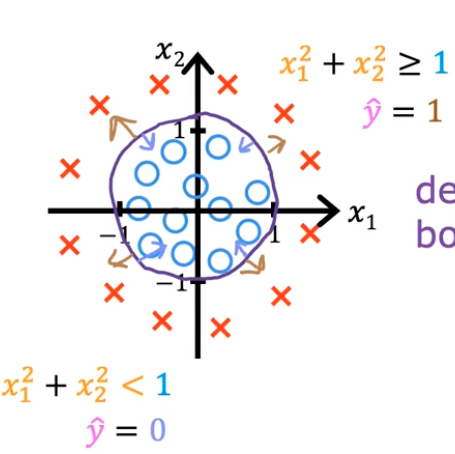
\includegraphics[height=5cm]{course_img/nonlinear_decision_boundary_ex}
\end{examplebox}

\newpage
\subsubsection{Cost function}

\begin{notebox}
	\begin{itemize}
		\item The squared error cost function is no longer a convex function to minimize for logistic regression model~\cref{eq:logistic_regression}.
		\item Can write the cost function in terms of the loss function~\cref{eq:loss_function} and this new cost function is a convex function to find a global minima for minimizing the model parameters.
		\item Below the concept underpoinning the equations for the cost function is \textbf{Maximum Likelihood estimation} 
	\end{itemize}
\end{notebox}

\begin{definitionbox}
	The \textbf{Cost function} for logistic regression can be written in terms of a loss function:
	\begin{equation}\label{eq:cost_function_regression_short}
		J(\vec{w},b) = \frac{1}{m} \sum \limits^{m}_{i=1} L \left( f_{\vec{w},b} (\vec{x}^{(i)}),y^{(i)}\right)
	\end{equation}
	where the \textbf{Logistic Loss function} tells us the likelihood (probability from 0 to1) of fitting the model well is defined as
	\begin{equation}\label{eq:loss_function}
		L\left( f_{\vec{w},b}(\vec{x}^{(i)}), y^{(i)}\right) = (-y^{(i)} \log\left(f_{\vec{w},b}\left( \vec{x}^{(i)} \right) \right) - \left( 1 - y^{(i)}\right) \log \left( 1 - f_{\vec{w},b}\left( \vec{x}^{(i)} \right) \right)
	\end{equation}
	and can be written for both cases:
	\begin{equation}\label{eq:loss_function_cases}
		L \left( f_{\vec{w},b} ( \vec{x}^{(i)},y^{(i)}\right) =
		\begin{cases}
			-\log \left( f_{\vec{w},b} (\vec{x}^{(i)}) \right) & \textit{if}\quad y^{(i)} = 1 \\
			-\log \left( 1 - f_{\vec{w},b} (\vec{x}^{(i)}) \right) & \textit{if}\quad y^{(i)} = 0.
		\end{cases}
	\end{equation}
	
	Finally the cost function can be rewritten by plugging in~\cref{eq:loss_function} into~\cref{eq:cost_function_regression_short}: 
	\begin{equation}\label{eq:cost_function_regression_long}
		\boxed{J(\vec{w},b) = -\frac{1}{m} \sum \limits^{m}_{i=1} \left[
(-y^{(i)} \log\left(f_{\vec{w},b}\left( \vec{x}^{(i)} \right) \right) - \left( 1 - y^{(i)}\right) \log \left( 1 - f_{\vec{w},b}\left( \vec{x}^{(i)} \right) \right)\right],}
	\end{equation}
	where this is the useful form for programing the loss for gradient decent.
\end{definitionbox}

\begin{examplebox}
	Example of cases for loss function determination:\\
	Case 1: $y^{(i)} = 1$, 
	\begin{itemize}
		\item As the model $f_{\vec{w},b} (\vec{x}^{(i)})\rightarrow 1$ the loss function $L\rightarrow 0$ and  the prediction is close to the true value ($L$ is small)
		\item Similarly as $f_{\vec{w},b} (\vec{x}^{(i)})\rightarrow 0$ $L\rightarrow \infty$ and penalizes the model to find a smaller loss
	\end{itemize} 
	
	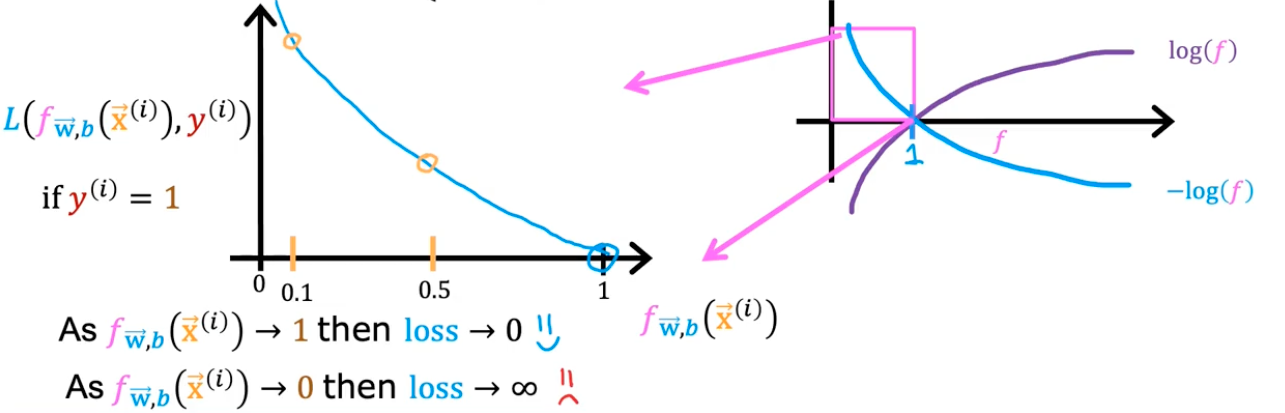
\includegraphics[width=\textwidth]{course_img/loss_function_ex}
	
	Case 2: $y^{(i)} = 0$,
	\begin{itemize}
		\item As the model $f_{\vec{w},b} (\vec{x}^{(i)})\rightarrow 0$ the loss function $L\rightarrow 0$ and the prediction is close to the true value ($L$ is small) penalizes the model to find a smaller loss 
		\item Similarly as $f_{\vec{w},b} (\vec{x}^{(i)})\rightarrow 1$, $L\rightarrow \infty$ and  penalizes the model to find a smaller loss 
	\end{itemize}
	
	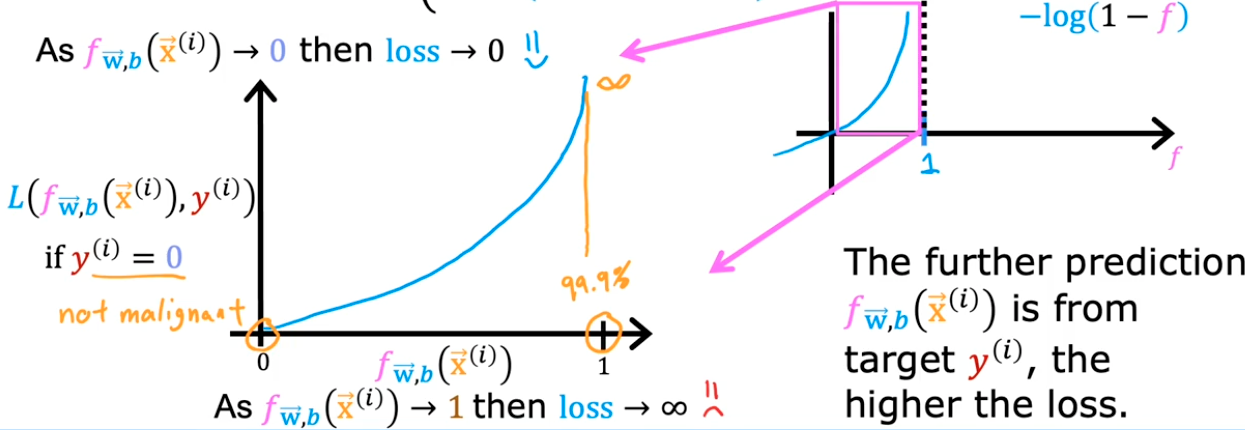
\includegraphics[width=\textwidth]{course_img/loss_function_ex2}
	
\end{examplebox}

\subsubsection{Gradient descent implementation}

\begin{notebox}
	The gradient decent algorithm for logistic regression can be calculated by using the definition for multiple features~\cref{eq:gradient_descent_multi} with the logistic regression model~\cref{eq:logistic_regression} where the derivative of the cost functions using~\cref{eq:cost_function_regression_long} is:
	\begin{align}
		\frac{\partial}{\partial w_j} J(\vec{w},b) &= \frac{1}{m} \sum \limits^{m}_{i=1} \left(
f_{\vec{w},b}( \vec{x}^{(i)} )  - y^{(i)}\right) x_i^{(i)},
	\\
		\frac{\partial}{\partial b} J(\vec{w},b) &= \frac{1}{m} \sum \limits^{m}_{i=1} \left(
f_{\vec{w},b} (\vec{x}^{(i)} ) - y^{(i)} \right), 	
	\end{align}
which looks similar to linear regression but $f_{\vec{w},b}( \vec{x}^{(i)} )$ is now the sigmoid function~\cref{eq:sigmoid}.
\end{notebox}

\subsection{Problem of overfitting }

The goal of machine learning regression is to find the model that fits the data just right.

\begin{definitionbox}
	When the data is \textbf{Underfit} or has \textbf{High Bias} the model does not fit the training set well,e.g., an oversimplified model to data \\
	
	 When the data is \textbf{Overfit} or has \textbf{High Variance} the model fits the data too well\\
	 -- can have instability of predictions (high variance) when training with slightly different training set(does not generalize well) \\
	 -- can model many features that are unrealistic in the data,e.g., the third image below shows a dip in the housing prices at the dotted magenta line which is inconsistent with the shape of the data \\
	 
	 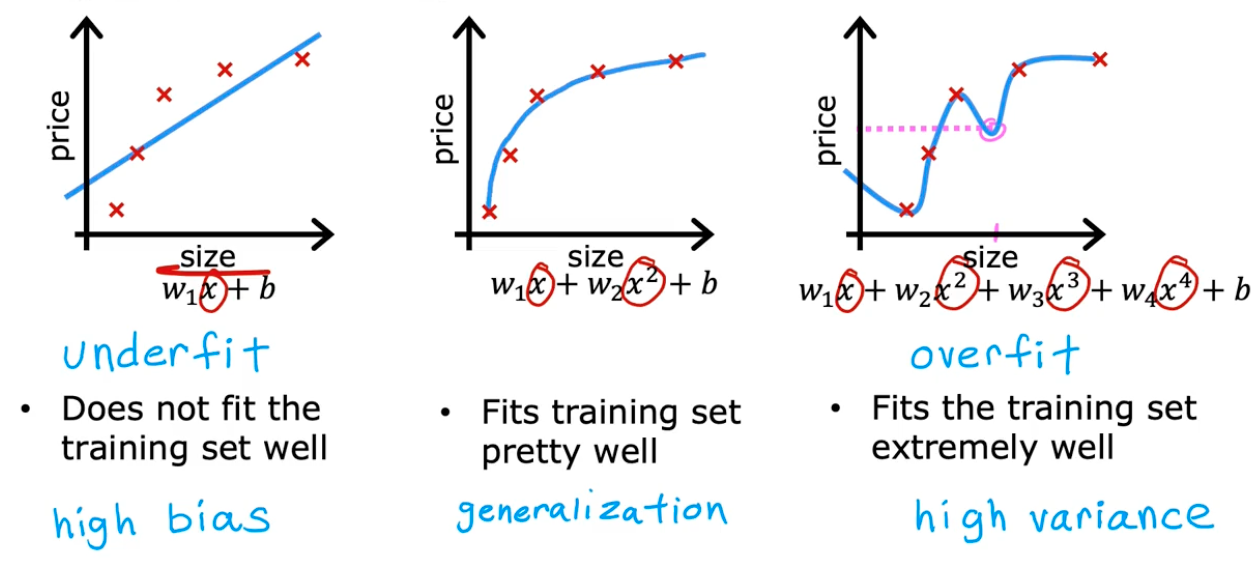
\includegraphics[width=\textwidth]{course_img/fitting_ex}
	 
\end{definitionbox}

\begin{examplebox}
	For this example, different logistic ergression models are used to classify the boundary function for finding a malignant tumor.
	\\
	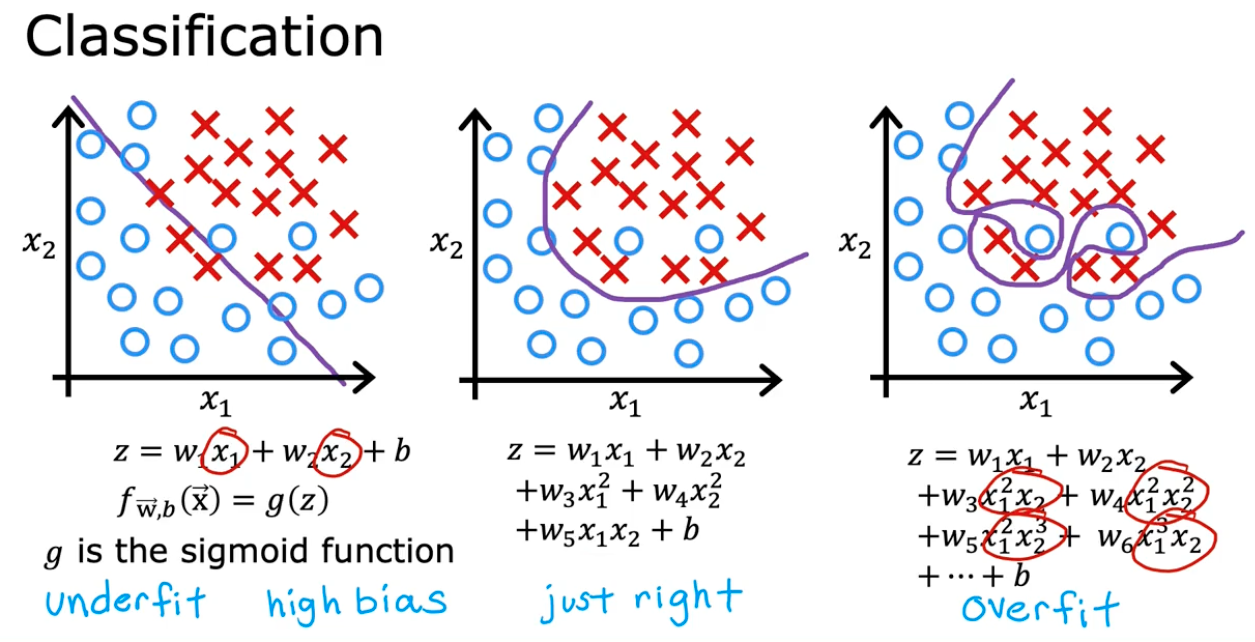
\includegraphics[height=5cm]{course_img/fitting_classification_ex}
	
\end{examplebox}

\subsubsection{Addressing the problem}

\begin{notebox}
	To address overfitting we can:
	\begin{itemize}
		\item  collect more training examples
		\item reduce/change the set of features used (simplify model), e.g., \textbf{Feature Selection} (discussed in course 2)
		\item  reduce the size of parameters,e.g., \textbf{Regularization} 
	\end{itemize}

\end{notebox}

\subsection{Regularization}
	
\begin{definitionbox}
	\textbf{Regularization} is used to reduce wights of features in our model without having to omit any features. \\ 
	The regularized cost function example using the squared errors cost function~(\cref{eq:cost_function} is modified by adding a constraining term(regularization term) introducing the \textbf{regularization parameter, ($\lambda$)}:
	\begin{equation}\label{eq:regularized_cost_function}
		J_{regularized}(\vec{w},b) = \frac{1}{2m} \sum\limits_{i=1}^m \left( f_w \left( x^{(i)} \right) - y^{(i)} \right)^2 + \frac{\lambda}{2m}\sum\limits_{j=1}^n w_j^2 + \left[  \frac{\lambda}{2m} b^2 \right]
	\end{equation}
	where $\lambda>0$ and the term to regularize $b$ may be excluded without drastically changing the result.\\
	-- The regularization term balances fitting the data well and keeping the weights $w_j$ of the model small. \\ 
	-- If $\lambda=0$ the model will  not reduce the weights and overfit the model. \\
	-- if $\lambda$ is too large the $w_j\rightarrow 0$ because of the big penalty when minimizing and underfit the model. \\ 
	
	[Note] This is similar to the Lagrange multipliers method used in least squares fitting in my research
\end{definitionbox}

\subsubsection{Regularized Regression with gradient descent}

\begin{notebox}
	The gradient decent algorithm for regularized linear regression can be written using~\cref{eq:regularized_cost_function} and using the definition of gradient decent~(\cref{eq:gradinet_descent_linear}) we just need the derivatives of the regularized cost function:
	\begin{align}
		\frac{\partial}{\partial w_j} J(\vec{w},b) &= \frac{1}{m} \sum \limits^{m}_{i=1} \left(
f_{\vec{w},b}( \vec{x}^{(i)} )  - y^{(i)}\right) x_i^{(i)} +\frac{\lambda}{m}w_j,
	\label{eq:regularized_gradient_descent} 
	\\ 
		\frac{\partial}{\partial b} J(\vec{w},b) &= \frac{1}{m} \sum \limits^{m}_{i=1} \left(
f_{\vec{w},b} (\vec{x}^{(i)} ) - y^{(i)} \right), 	
	\end{align}
	
	\textbf{Deeper Dive}\\
	If we plug these derivatives back into the gradient decent~(\cref{eq:gradinet_descent_linear}) and factor out and isolate $w_j$ in~\cref{eq:regularized_gradient_descent} then we can rewrite it the updated parameters as:
	\begin{equation}
		w_j^{new} = w_j \left( 1-\alpha\frac{\lambda}{m} \right) -\alpha \frac{1}{m} \sum \limits^{m}_{i=1} \left(f_{\vec{w},b}( \vec{x}^{(i)} )  - y^{(i)}\right) x_i^{(i)}
	\end{equation}
	where we can see that the regularization just shrinks the original parameter by a factor of ($\alpha\frac{\lambda}{m}$) and the second term is the normal update without regularization.
	
	Very generally the above procedure can be used for logistic regression where the cost function is now~\cref{eq:cost_function_regression_long}.
\end{notebox}

\subsection{Summary}



\end{document}
